%!TEX root = ../BPlusTree-report.tex
\section{Background}
\label{sec:Background}
% Notes:
% What is a bplustree:
%   - Inherently imperative data structure
%   - Suboptimal implementation
%     - Running time of optimal implementation
%     - Running time of our implementation
%       - Mention how one could make it optimal.
%       - A tree in a tree in a tree, dawg
%     - Running time out of scope

\subsection{Gallina}
Gallina is a purely functional language\todo{ref}, which is used by the Coq interactive proof assistant. It is very lean, and does not include non-functional data structures, such as arrays\todo{ref}.

\subsection{B+ tree}
The B+ tree is a n-ary, self-balancing, tree data structure\todo{ref}, similar to a B-tree\todo{ref}. It is composed of a root, nodes, and leaves. The root may be a leaf or a node. Nodes hold pairs of keys and pointers, $(k, p)$. $p$ points to either a node or leaf that holds the values over $k$, but below the key of the next pair. Leaves hold pairs of keys and values, $(k, v)$. In this project keys are always natural numbers, while values can have any type, denoted by $X$. 

\begin{figure}
 \centering
   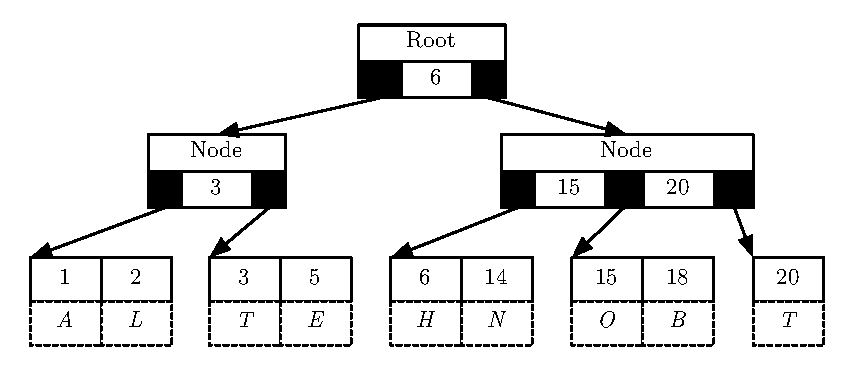
\includegraphics[width=90mm]{diagrams/BPlusTree.pdf}
 \caption{An example of a B+ tree with $b=2$. The bottom row contains leaves, with values, in this case characters, in the dashed boxes.}
 \label{fig:bplustree}
\end{figure}

For a given B+ tree, a branching factor $b$
leaves\todo{ref}. A node must have at least $b/2$ children, and at most $b$. A
leaf must have between $b/2$ and $b$ values. This rule is relaxed for the root
node, which must have between 2 and $b$ children. \todo{For nodes and 0 - 2*b for leaves}

\paragraph{}
In our implementation, a node is a list of key-pointer $(k, p)$ pairs where $p$ points to a child tree. A leaf is a list of key-value $(k, v)$ pairs. We support three operations, which we will refer to as our primary operations. These are: insert, search and height. The theory behind the height function is trivial, and will not be explained in this section, but the theory behind the insertion and search functions require some explanation. Beyond these primary operations, we have also implemented a simple in-order traversal, which we will not cover in this report.

\subsubsection{Insert}


\subsubsection{Search}
The search function takes two arguments: a search key $sk$, and a tree $t$, to search in. Tree can be either a node or a leaf. If the the tree is a node, the function recurses through the $(k, p)$ list, until it finds the pair $(k, p)$, value where $k \le sk$, and $sk < k1$, where $k1$ is the following pair $(k1, p1)$ in the list. The function then recursively calls itself with the subtree $p$. Once the function reaches a leaf, the $(k, v)$ list is searched, for example by doing a binary search.
